\chapter{Case Study}\label{ch:case-study}

In December 2019, a virus known as COVID-19 was first identified in Wuhan, China~\cite{seznamKorona2021}.
Three months later, on March 1, 2020, the first three cases of the disease were confirmed in the Czech Republic~\cite{seznamKorona2021}.
The disease has shown and continues to show the shortcomings of social and political environment worldwide.
But the disease, although very serious, has given us many opportunities.
One such opportunity is open datasets made available by state institutions.

In the following part of the work we will try to analyze the state of datasets provided by the institutions of the Czech Republic.
We apply the metrics defined in Chapter 3 to the data in order to objectively measure their quality and comment on the results.
Available datasets as of April 1, 2020 from the URL address \url{https://onemocneni-aktualne.mzcr.cz/} are listed in Appendix~\ref{ch:dataset-collection}.

\section{Technical Analysis}

The data can be downloaded via the REST API in JSON, in addition, the data can be downloaded in CSV together with metadata also in JSON format.
The format of the JSON data file can be seen in Figure~\ref{ls:data}.
All data files contain one main object, with three keys (modified, source and data).
The \enquote{modified} key contains the date of the dataset update in ISO 8601 format with the time offset from UTC (Coordinated Universal Time).
The \enquote{source} key contains the URL of the dataset, especially the protocol and domain name.
The last key, the data, contains an array of json objects with a structure given by the metadata.
This is an array of objects even if the array contains only one object.

\begin{figure}[htb]
    \centering
    
    \begin{lstlisting}[language=json,firstnumber=1]
{
    "modified": "2021-04-18T12:28:42+02:00",
    "source": "https:\/\/onemocneni-aktualne.mzcr.cz\/",
    "data": [
        {
            ...
        }
    ]
}
    \end{lstlisting}

    \caption{Data file structure}
    \label{ls:data}
\end{figure}
\FloatBarrier

An example of the structure of the metadata file can be found in the appendix~\ref{ch:metadata-file-structure}.

\section{Data Analysis}

One of the most serious errors in the data catalog is the absence of categorization of deaths.
% V datasetu, obsahujícím data o úmrtí pacientů, se dozvíme datum úmrtí, věk pacienta, pohlaví a kódy kraje a obce ze kterého pacient pocházel.
In the dataset, which contains data on patients' deaths, we learn the date of death, the patient's age, gender and the codes of the region and municipality from which the patient came.
It does not take into account whether the patient was very ill (e.g., a patient with pancreatic cancer in advanced metastasis) or generally polymorbid (i.e., having number of illnesses) and therefore had a high probability of death, or if the patient was a completely healthy person.
No consideration of this fact leads to the introduction of virtually immeasurable systematic error.

\begin{figure}[htb]
    \centering
    
    \begin{lstlisting}[language=json,firstnumber=1]
[
    {
    "datum": "2020-01-01",
    "vek": 50,
    "pohlavi": "M",
    "kraj_nuts_kod": "CZ000",
    "okres_lau_kod": "CZ0000"
    },...
]
    \end{lstlisting}

    \caption{Sample data with information on deceased patients}
    \label{ls:sample-data-deceased}
\end{figure}
\FloatBarrier

A similar issue can be observed in the data on new COVID-19 cases and the daily number of tests performed.
In the first case we are unable to determine whether there are any percentage of patients in whom the disease manifested itself repeatedly.
In the second case, information on retested patients is missing.
All these problems lead to a reduction in data quality, which we are not able to measure effectively.

Another factor reducing the quality is the methodology itself.
According to the methodology, a person is considered cured since the last negative test.
However, it does not take into account whether this person is still in the intensive care unit with post-COVID syndrome or whether he is really cured.

Spíše ekonometrická data

\begin{figure}[htb]
    \centering
    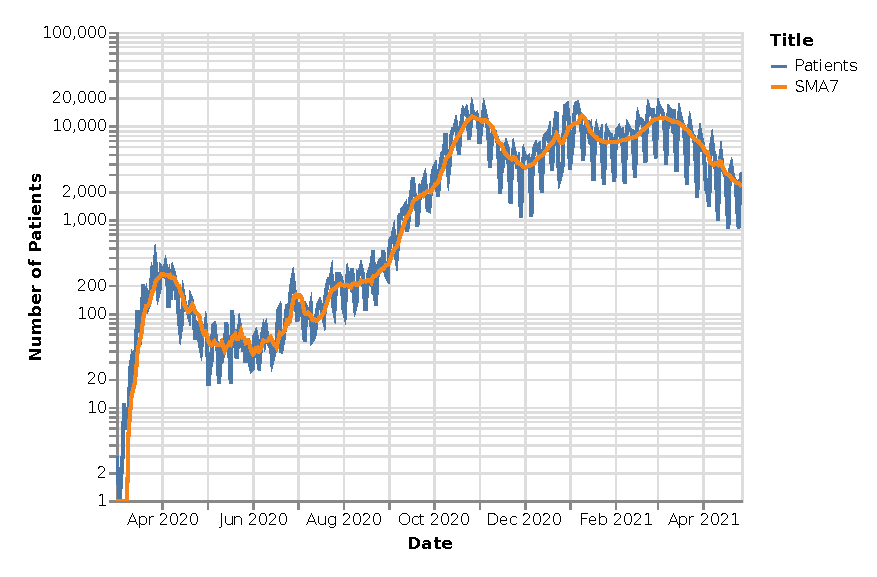
\includegraphics[width=0.9\textwidth]{figures/recovered-sma7.eps}
    \caption{Daily confirmed cases of infection and weekly moving average.}
    \label{fig:recovered-sma7}
\end{figure}
\FloatBarrier

